\subsection{Клиентская часть}
Разработка клиентской части начинается с проектирования развернутой и полной диаграммы классов, которая отражает взаимодействие между внутренними частими, в частности графической оболочкой и классом, реализующим внутренний интерфейс. 
Также в этой части рассмотрен непосредственно пользовательский интерфейс.То есть рассматиривается уже диаграмма классов с точки зрения реализации, а не концептуальной, как было в первой части работы.

Диаграмма классов (Class diagram)~-- статическая структурная диаграмма, описывающая структуру системы, она демонстрирует классы системы, их атрибуты, методы и зависимости между классами.

\begin{figure}[ht]
\centering
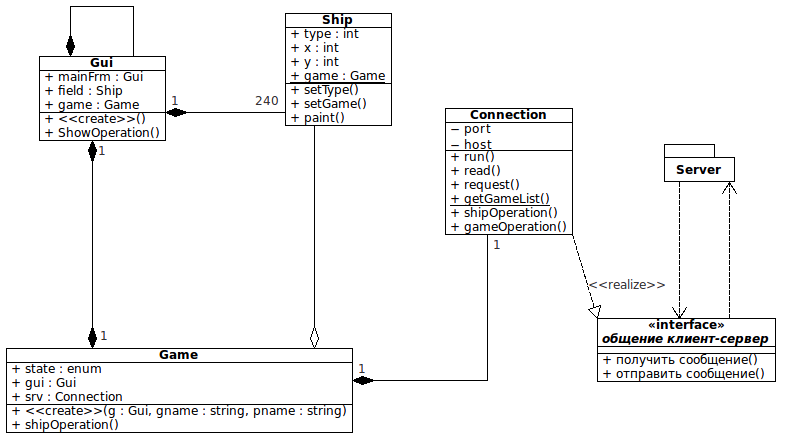
\includegraphics[width=18cm]{images/class_client.png}
\caption{Диаграмма классов клиента}
\label{fig8}
\end{figure}


Анализ правил и условий игры показал, что, для упрощения реализации, необходимо выделить класс Ship, который будет отвечать за отрисовку кораблей на поле и действия кораблей при клике мышкой на них.

Класс Game будет являться прослойкой между классом и Графическим интерфейсом(Gui). Рассмотрим работу интерфейса на примере создания игры[\ref{fig9}]. В дальнейших описаниях класс Connect будет опускаться, так как является частью внутреннего взаимодействияклиента и сервера, что рассматривалось в предыдущей главе.

\begin{figure}[pt]
\centering
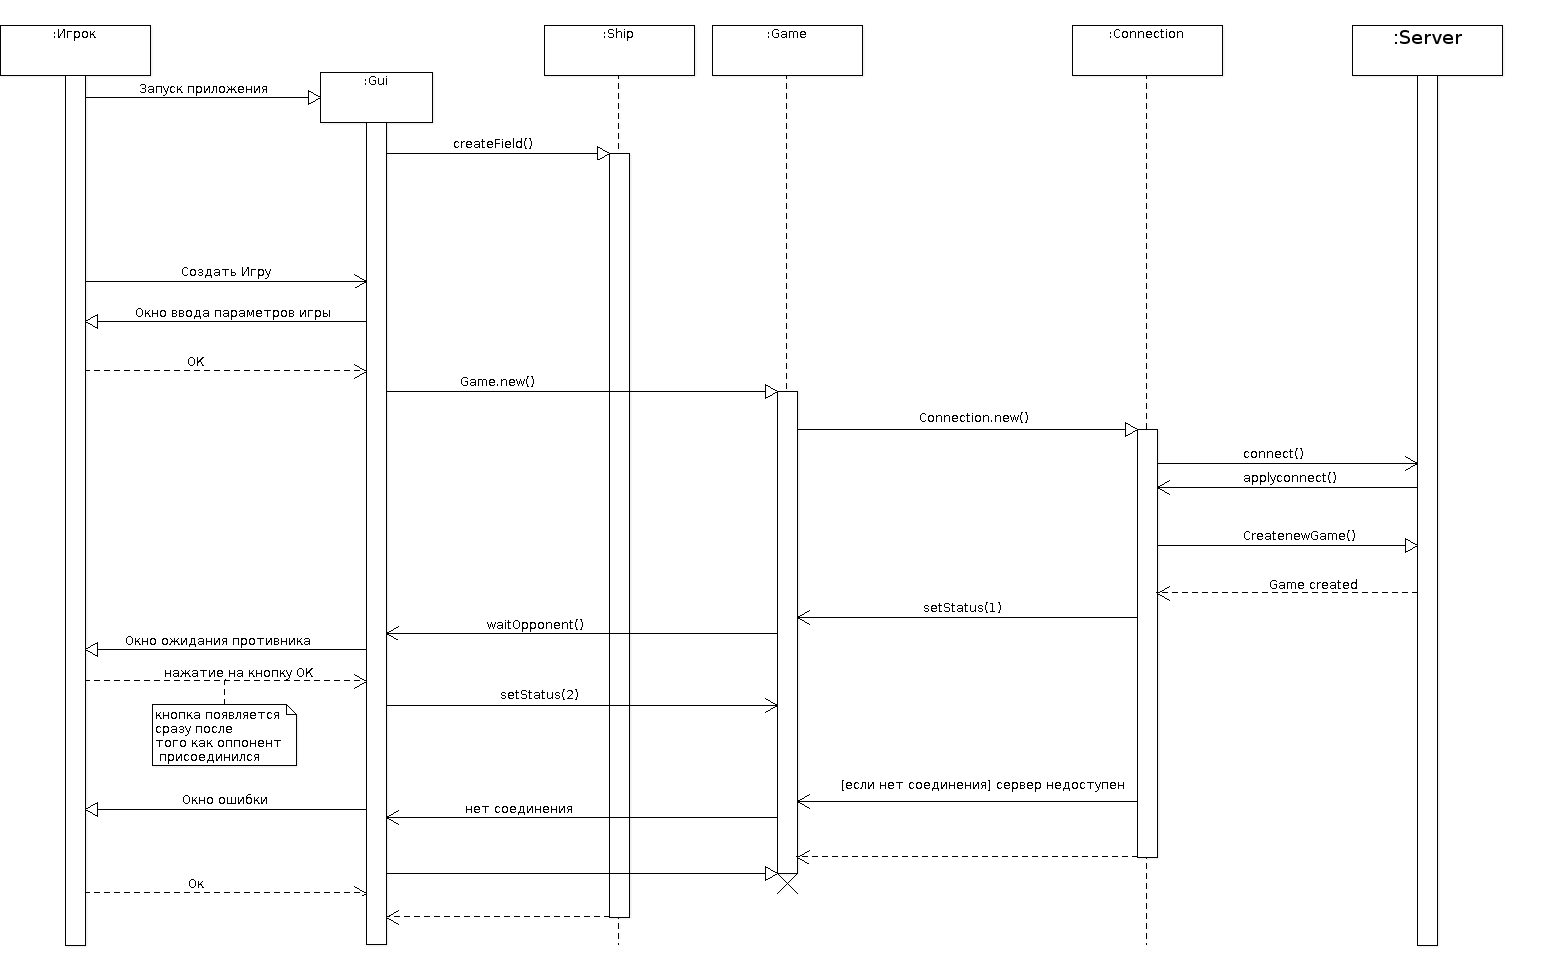
\includegraphics[width=15cm]{images/CRG.png}
\caption{Диаграмма создания новой игры}
\label{fig9}
\end{figure}

\newpage
Ещё один аспект, который был включен на диаграмме[\ref{fig0}] в вариант использования <<Управление игрой>> это присоединение к игре, созданной другим игроком. Взаимодействие классов между собой при этом прецеденте показано на схеме[\ref{fig10}].

\begin{figure}[pt]
\centering
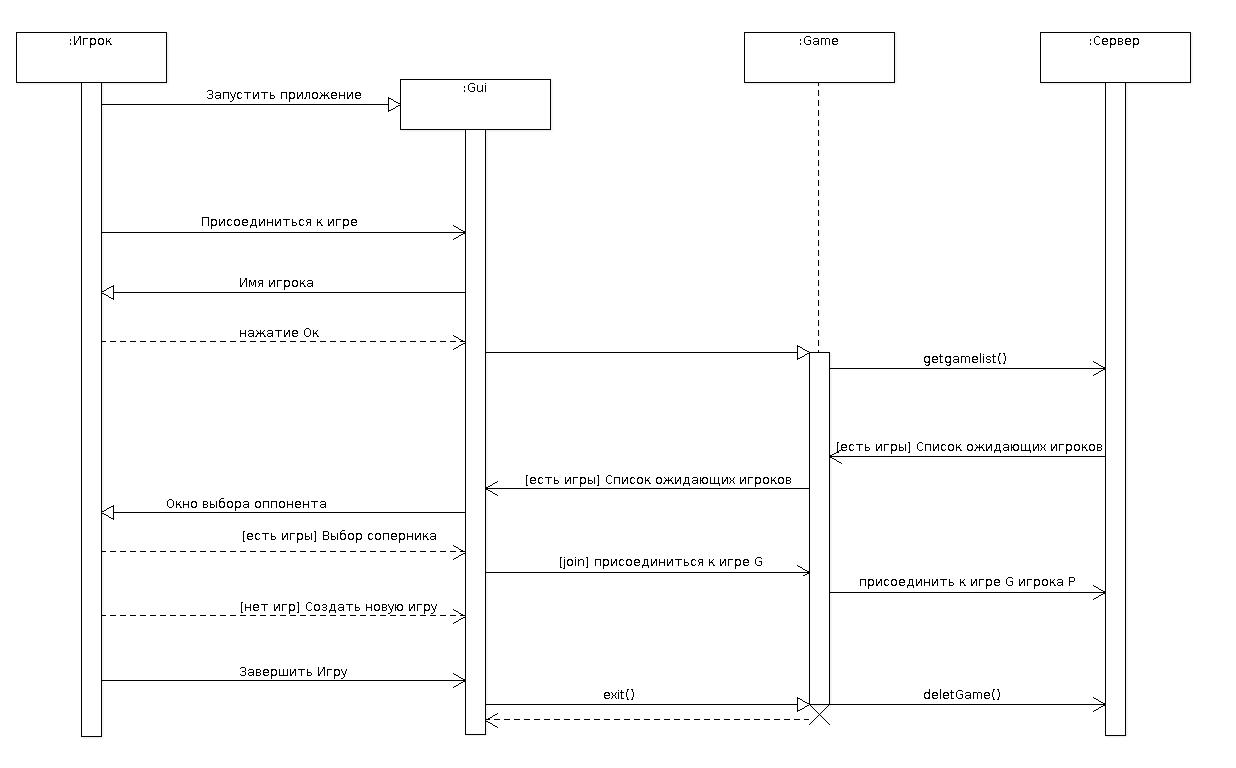
\includegraphics[width=18cm]{images/JG.png}
\caption{Диаграмма присоединения к игре}
\label{fig10}
\end{figure}

Действия, производимые над объектом класса Ship в течение всего процесса иры:
	\begin{itemize}
		\item Расстановка кораблей перед боем;
		\item Передвижение корабля;
		\item Вопрос к корабляю противника;
		\item Ответ на вопрос корабля противника;
		\item Взрыв бомбы;
		\item Взрыв торпеды;
  	\end{itemize} 
Естесственно не все эти вариатнты следует отображать на диаграммах, так как многие из них сводятся к реализации простейших функций и не требуют детального проектирования. Рассмотрим наиболее интересные, например расстановку кораблей, части которой можно использовать не только при форминовании начального игрового поля, но и при описании процесса снятия и пережвижения кораблей во время матча[\ref{fig11}].

\begin{figure}[pt]
\centering
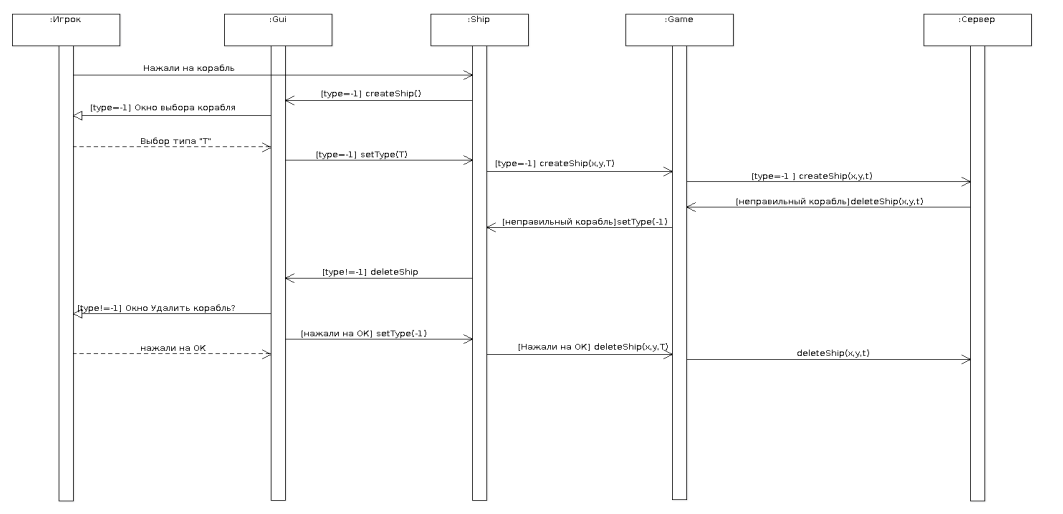
\includegraphics[width=18cm]{images/CRS.png}
\caption{Диаграмма установки корябля}
\label{fig11}
\end{figure}

Игра проходит в несколько этапов. Действия игрока зависят от того какой этап игры идет. Зависимость между этапами игры и действиями, которые предшествуют тому или иному состоянию игры можно увидеть на диаграмме[\ref{fig11}].

\begin{figure}[ht]
\centering
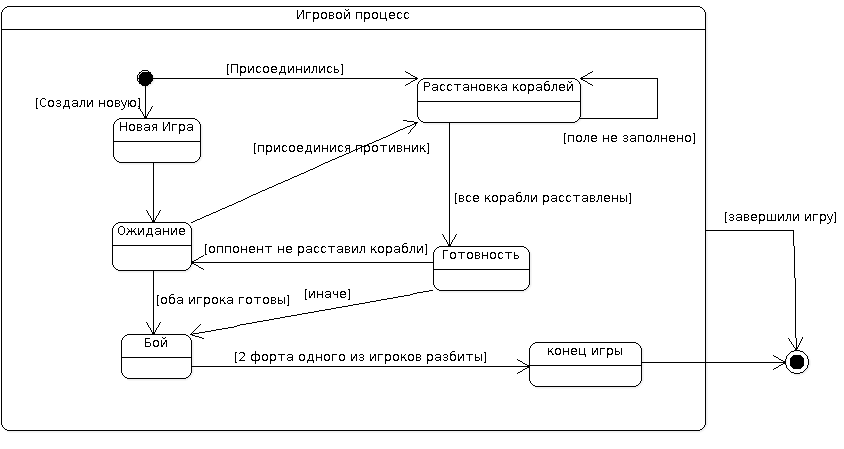
\includegraphics[width=18cm]{images/statecl.png}
\caption{Диаграмма состояний игры}
\label{fig12}
\end{figure}


Следует подчеркнуть, что состояние <<Бой>> на [\ref{fig12}] раскрыто не полностью, так как есть небольшие подсостояния, зависящие например от очередности хода или совершаенго действия из списка возможных, которые тоже можно выделять в отдельные состояния. Они будут рассмотрены в следующей части, так как относятся к правилам, контролируемым сервером. 
\endinput
